\documentclass{standalone}
\usepackage{tikz}
\usepackage{xcolor}
\usetikzlibrary{decorations.markings}

\centering

\begin{document}
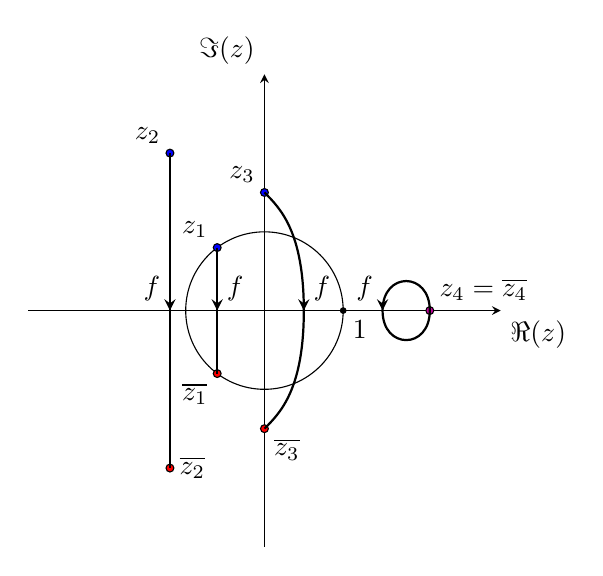
\begin{tikzpicture}[>=stealth]
    \tikzset{
    every node/.style={font=\normalsize, text=black},
    arrowstyle/.style={->, >=stealth}}
    %Assen
    \draw [->](0,-3) -- (0,3) node[above left]{$\Im(z)$};
    \draw [->](-3,0) -- (3,0) node[below right]{$\Re(z)$};
    
    %Eenheidscirkel
    \draw (0,0) circle(1);
    \draw[fill=black] (1,0) circle (1pt);
    \node[below right] at (1,0) {1};
    
    %coordinaten
    \coordinate (a1) at (0,1.5);
    \coordinate (a3) at (0,-1.5);
    \coordinate (a2) at (2.1,0);
    \coordinate (z1) at (-0.6, 0.8);
    \coordinate (z2) at (-1.2,2.0);
    \coordinate (z3) at (-0.6,-0.8);
    \coordinate (z4) at (-1.2,-2.0);

    
    
    
    %z
    \draw[fill=blue] (z1) circle(0.05) node[above left] {$z_1$};
    \draw[fill=blue] (z2) circle(0.05) node[above left] {$z_2$};
    \draw[fill=blue] (a1) circle(0.05) node[above left] {$z_3$};
    \draw[fill={rgb,255:red,196; green,0; blue,156}] (a2) circle(0.05) node[above right] {$z_4=\overline{z_4}$};
    %conjugate
    \draw[fill=red] (z3) circle(0.05) node[below left] {$\overline{z_1}$};
    \draw[fill=red] (z4) circle(0.05) node[right] {$\overline{z_2}$};
    \draw[fill=red] (a3) circle(0.05) node[below right] {$\overline{z_3}$};
    
    % Pijl van z naar conjugate(z)
    \draw[thick,postaction={decorate}, decoration={markings,mark=at position 0.5 with {\arrow{stealth}}}]
    [black] (a1)
    .. controls (0.2,1.3) and (0.5,1) .. (0.5,0)
    .. controls (0.5,-1) and (0.2,-1.3) .. (a3);
    \node[above right,black] at (0.5,0) {$f$};
    
    \draw[thick,postaction={decorate}, decoration={markings,mark=at position 0.5 with {\arrow{stealth}}}]
    [black] (a2)
    .. controls (2.1,0.5) and (1.5,0.5) .. (1.5,0)
    .. controls (1.5,-0.5) and (2.1,-0.5) .. (a2);
    \node[above left,black] at (1.5,0) {$f$};
    
    \draw[thick,postaction={decorate}, decoration={markings,mark=at position 0.5 with {\arrow{stealth}}}]
    [black] (z2)
    .. controls (-1.2,0.3) and (-1.2,0.3) .. (-1.2,0)
    .. controls (-1.2,-0.3) and (-1.2,-0.3) .. (z4);
    \node[above left,black] at (-1.2,0) {$f$};
    
    \draw[thick,postaction={decorate}, decoration={markings,mark=at position 0.5 with {\arrow{stealth}}}]
    [black] (z1)
    .. controls (-0.6,0.3) and (-0.6,0.3) .. (-0.6,0)
    .. controls (-0.6,-0.3) and (-0.6,-0.3) .. (z3);
    \node[above right,black] at (-0.6,0) {$f$};

\end{tikzpicture}
\end{document}